We adapt the framework in \citet{kim2022influencing} to the partially observable setting and formalize the problem of multi-agent learning as a Partially Observable Active Markov Game with periodic policy updates. Throughout the paper, we will use the bold convention to denote the collection of joint sets, joint variables and joint functions for $i \in I =\{1,\ldots,n\}$, where $\boldsymbol{X} := \times_{i \in I} X^i$ for set $X^i$, $\boldsymbol{x} := \{x_1, \ldots, x_n\}$ for variable $x^i$ and $\boldsymbol{G}(\cdot) := \prod_{i \in I} G^i(\cdot)$ for function $G^i(\cdot)$.

\section{Partially Observable Active Markov Games}
In social learning environments, agents rarely possess complete information about the underlying state of the world. Instead, they receive private signals—often limited and noisy—that only partially reveal the true state, while also observing the actions of other participants rather than their private information. This fundamental information asymmetry is a cornerstone of economic models of social learning. The challenge of inferring valuable information from others' actions while acknowledging the confounding influence of their own social learning creates rich strategic dynamics that cannot be captured by frameworks assuming full observability. This necessitates extending our theoretical approach to the partially observable setting. Standard approaches to partial observability, such as Partially Observable Markov Decision Processes (POMDPs) and Decentralized POMDPs, address this challenge in single-agent and cooperative multi-agent contexts respectively. However, these frameworks do not adequately capture the strategic nature of policy evolution that characterizes the social learning environments, and neither do they allow for flexible modeling of the reward functions. Building on the Active Markov Game formulation of \citet{kim2022influencing}, we introduce Partially Observable Active Markov Games (POAMGs), which integrate belief state dynamics with evolving policy parameters to model sophisticated social learning dynamics under uncertainty.

\begin{definition}[Partially Observable Active Markov Game]
    A Partially Observable Active Markov Game is defined as a tuple $M_n = \langle I, S, \boldsymbol{A}, T, \boldsymbol{O}, \boldsymbol{R}, \boldsymbol{\Theta}, \boldsymbol{U} \rangle$, where:
    \begin{itemize}
        \item $I = \{1, \ldots, n\}$ is the set of $n$ agents;
        \item $S$ is the state space, assumed to be discrete and finite;
        \item $\boldsymbol{A} = \times_{i \in I} A^i$ is the joint action space, where $A^i$ is the action space of agent $i$;
        \item $T: S \times \boldsymbol{A} \mapsto \Delta(S)$ is the Markovian state transition function, with $T(s'|s, \boldsymbol{a})$ denoting the probability of transitioning to state $s'$ after taking joint action $\boldsymbol{a}$ in state $s$;
        \item $\boldsymbol{O} = \times_{i \in I} O^i$ is the joint observation function, with $O^i: S \times \Omega^i \mapsto \Delta(\Omega^i)$ denoting the observation function for agent $i$ and $\Omega^i$ denoting the observation space for agent $i$;
        \item $\boldsymbol{R} = \times_{i \in I} R^i$ is the joint reward function, with $R^i: S \times \boldsymbol{A} \mapsto \mathbb{R}$ denoting the reward function for agent $i$;
        \item $\boldsymbol{\Theta} = \times_{i \in I} \Theta^i$ is the joint policy parameter space, where $\Theta^i$ is the policy parameter space for agent $i$;
        \item $\boldsymbol{U} = \times_{i \in I} U^i$ is the joint Markovian policy update function, with
              $U^i: \Theta^i \times O^i \times \boldsymbol{A} \times R^i \times O^i \mapsto \Delta(\Theta^i)$ denoting the policy update function for agent $i$.
    \end{itemize}
\end{definition}
This formulation extends the Active Markov Game framework by incorporating observation functions that mediate agents' perceptions of the environment state. Next, we define policies of the agents based on their beliefs about the underlying state of the environment.

\begin{definition}[Belief-Based Policy]
    Under partial observability, each agent $i$ maintains a belief state $b_t^i \in B^i$ at time $t$, representing its probability distribution over states given its observation history. The policy of agent $i$ is defined as a mapping from belief and parameter spaces to distributions over actions:
    \begin{equation}
        \pi^i: B^i \times \Theta^i \mapsto \Delta(A^i)
    \end{equation}

    where $\pi^i(a^i|b^i; \theta^i)$ represents the probability of agent $i$ taking action $a^i$ given belief state $b^i$ and policy parameters $\theta^i$.
\end{definition}
\iffalse
The figure below illustrates the structure of the POAMG framework, highlighting the interplay between states, observations, beliefs, and policy parameters.

\begin{figure}[htb]
    \centering
    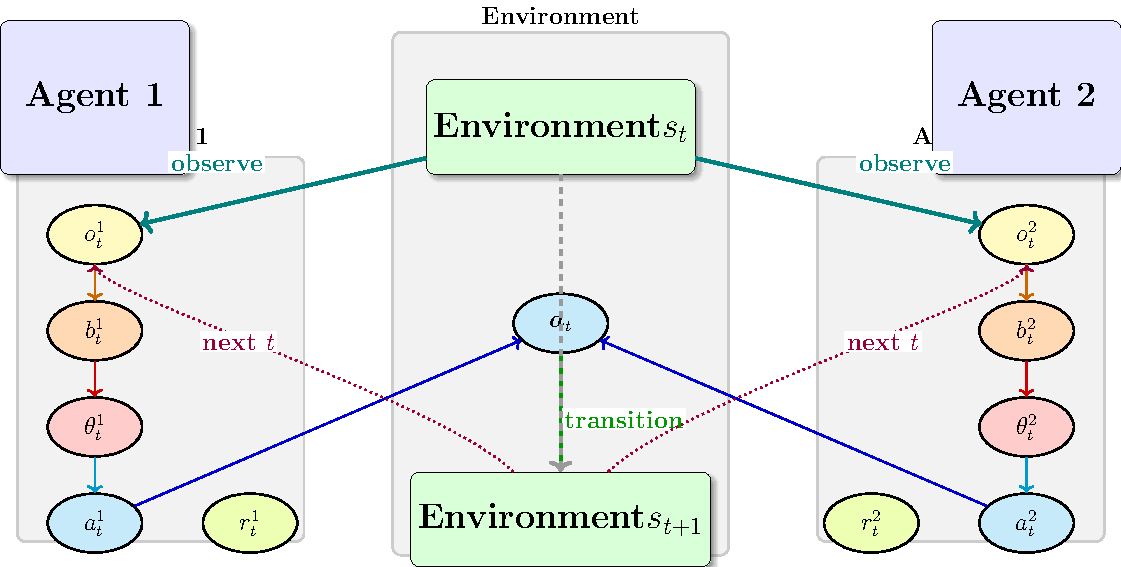
\includegraphics[width=0.9\linewidth]{figures/poamg-structure.pdf}
    \caption{Structure of a POAMGshowing the relationships between environment state, observations, beliefs, and policy parameters in a two-agent setting.}
    \label{fig:poamg-structure}
\end{figure}
\fi

In partially observable active Markov games, agents form beliefs to infer the underlying state of the environment. Unlike standard partially observable settings, these states evolve through the dynamically changing policies of the agents in addition to the environmental dynamics. The process unfolds as follows: at time step $t$, each agent $i$ selects an action at state $s_t \in S$ by sampling from its belief-conditioned policy $a^i_t \sim \pi^i(\cdot|b^i_t; \theta^i_t)$. When all agents act collectively through joint action $\boldsymbol{a_t}$, the environment transitions from $s_t$ to $s_{t+1}$ with probability $T(s_{t+1}|s_t, \boldsymbol{a}_t)$. Subsequently, each agent $i$ receives a reward $r^i_t = R^i(s_t, \boldsymbol{a}_t)$ and adjusts its policy parameters via the update function $U^i(\theta^i_{t+1}|\theta^i_t, \tau^i_t)$, where $\tau^i_t = \{o_t^i, \boldsymbol{a_t}, r^i_t, o_{t+1}^i\}$ is the trajectory for agent $i$ at time $t$ consisting of the current observation $o_t^i$, joint action $\boldsymbol{a_t}$, reward received $r^i_t$, and the next observation $o_{t+1}^i$. This adaptive cycle continues until non-stationary policies reach convergence. A key insight is that the joint policy update function $\boldsymbol{U}$ depends on $a^i_t$, which directly impacts state transitions and rewards, thereby enabling agent $i$ to strategically shape future collective policies through its individual decisions. This explicit modeling of strategic influence constitutes the primary advantage of active Markov games over their stationary counterparts.

\section{Convergence}
A central question in our analysis is whether the joint process of states, beliefs and policy parameters converges to a well-defined stationary distribution, and under what conditions. Following \citet{kim2022influencing}, we establish this connection using the properties of regularly perturbed Markov processes. First, we define the joint process, which operates on the joint space of states, beliefs and policy parameters.

\begin{definition}[Joint Process]
    In a Partially Observable Active Markov Game, the joint process $(s_t, \boldsymbol{b}_t, \boldsymbol{\theta}_t)$ consists of the state $s_t \in S$, the joint belief state $\boldsymbol{b}_t = (b^1_t, \ldots, b^n_t) \in \boldsymbol{B}$ and joint policy parameters $\boldsymbol{\theta}_t = (\theta^1_t, \ldots, \theta^n_t) \in \boldsymbol{\Theta}$ of all agents at time $t$.
\end{definition}
We then make the following assumptions on the subprocesses to ensure the ergodicity of the perturbed joint process.
\begin{assumption}[Communicating State Transition]\label{assumption:1}
    The state transition $T$ is communicating, meaning that for any two states $s, s' \in S$, there exists a sequence of joint actions $\boldsymbol{a}_1, \boldsymbol{a}_2, \ldots, \boldsymbol{a}_k$ and a sequence of states $s_1, s_2, \ldots, s_{k-1}$ such that:
    \begin{align}
        T(s_1|s, \boldsymbol{a}_1) > 0, \quad T(s_2|s_1, \boldsymbol{a}_2) > 0, \quad \ldots, \quad T(s'|s_{k-1}, \boldsymbol{a}_k) > 0
    \end{align}
\end{assumption}

\begin{assumption}[Communicating Belief-State Process]\label{assumption:2}
    The belief-state process is communicating, meaning that for any two belief states $b^i, b'^i \in B^i$, there exists a sequence of joint actions $\boldsymbol{a}_1, \boldsymbol{a}_2, \ldots, \boldsymbol{a}_m$ and a sequence of observations $o^i_1, o^i_2, \ldots, o^i_m$ such that:
    \begin{align}
        \mathbb{P}(b^i_{t+m} = b'^i | b^i_t = b^i, \boldsymbol{a}_t = \boldsymbol{a}_1, o^i_{t+1} = o^i_1, \ldots, \boldsymbol{a}_{t+m-1} = \boldsymbol{a}_m, o^i_{t+m} = o^i_m) > 0
    \end{align}
\end{assumption}
Assuming the communicating property of the subprocesses, we can establish convergence of the perturbed joint process to the unique stochastically stable distribution of the unperturbed one, as the perturbation vanishes in the limit.
\begin{theorem}[Stochastically Stable Distribution]
    Under Assumptions \ref{assumption:1} and \ref{assumption:2}, as $\epsilon \to 0$, the perturbed joint processes defined by $\epsilon$-perturbed policy update functions converge to the unique stochastically stable distribution $\mu^*$ of the unperturbed joint process $(s_t, \boldsymbol{b}_t, \boldsymbol{\theta}_t)$.
\end{theorem}

\begin{proof}
    See Appendix \ref{appendix:stochasticallystable} for a detailed proof.
\end{proof}
This convergence result has profound implications for our framework. By establishing the existence of a unique stochastically stable distribution, we provide a solid theoretical foundation for defining optimization objectives and analyzing equilibrium behavior in partially observable active Markov games. The stochastically stable distribution represents the limiting behavior of the system, independent of initial conditions, allowing us to characterize the long-run outcomes of social learning processes. This property is crucial for developing algorithms that optimize for long-term performance rather than myopic rewards, aligning with our goal of modeling sophisticated social learning dynamics.

\section{Incentives}
We now formalize the optimization objectives for agents in our Partially Observable Active Markov Game framework. In contrast to traditional reinforcement learning settings that typically employ discounted rewards, we first focus on the average reward criterion as our fundamental optimization objective.
The average reward formulation provides several compelling advantages for modeling social learning dynamics. As \citet{sutton2018reinforcement} emphasize, this approach is particularly well-suited for continuing tasks without natural episode boundaries—a characteristic that aligns perfectly with the ongoing nature of social learning interactions. While economic theory has predominantly employed discounted reward objectives due to their mathematical tractability and natural correspondence to time preference in utility maximization \citep{koopmans1960stationary, stokey1989recursive}, the average reward paradigm better captures the strategic considerations in our framework.
The key advantage of the average reward approach in our context is its emphasis on the limiting behavior of the multi-agent system. When agents engage in repeated strategic interactions over indefinite horizons, their primary concern becomes the long-run system behavior rather than transient dynamics. Moreover, unlike discounted objectives that can induce myopic behavior depending on the discount factor, the average reward formulation naturally encourages agents to consider the permanent effects of their actions on other agents' learning processes—a crucial aspect for accurately modeling the strategic dimensions of social learning.

\begin{definition}[Average Reward Objective under Partial Observability]
    Each agent $i \in I$ in a Partially Observable Active Markov Game aims to find policy parameters $\theta^i$ and update function $U^i$ that maximize its expected average reward $\rho^i \in \mathbb{R}$ based on the joint beliefs $\boldsymbol{b}$:
    \begin{align}
        \begin{split}
            \max_{\theta^i, U^i} \rho^i(\boldsymbol{b}, \boldsymbol{\theta}, \boldsymbol{U}) : & = \max_{\theta^i, U^i} \lim_{T \to \infty} \mathbb{E}\left[\frac{1}{T}\sum_{t=0}^T R^i(s_t, \boldsymbol{a}_t) \Bigg|
                \begin{array}{c}
                    \boldsymbol{b}_0= \boldsymbol{b}, \boldsymbol{\theta}_0= \boldsymbol{\theta}, \\
                    \boldsymbol{a}_t \sim \boldsymbol{\pi}(\cdot|\boldsymbol{b_t}; \boldsymbol{\theta_t}),
                    s_{t+1} \sim T(\cdot|s_t, \boldsymbol{a}_t),        \\
                    \boldsymbol{o}_{t+1} \sim \boldsymbol{O}(\cdot|s_{t+1}),
                    \boldsymbol{\theta}_{t+1} \sim \boldsymbol{U}(\cdot|\boldsymbol{\theta_t}, \boldsymbol{\tau_t})
                \end{array}
            \right]                                                                                                                                                                                                                                                                                                                          \\
                                                                                               & = \max_{\theta^i, U^i} \sum_{s, \boldsymbol{b}, \boldsymbol{\theta}} b^i(s) \mu^*(s, \boldsymbol{b}, \boldsymbol{\theta}) \sum_{\boldsymbol{a}} \boldsymbol{\pi}(\boldsymbol{a}|\boldsymbol{b}; \boldsymbol{\theta}) R^i(s, \boldsymbol{a})
        \end{split}
    \end{align}


\end{definition}

This formulation emphasizes that agents aim to maximize their rewards in the limiting behavior of the Markov process, focusing on long-term performance rather than immediate gains. The second equality expresses the objective in terms of the stochastically stable distribution $\mu^*$, weighted by agent's belief, connecting our optimization problem to the theoretical results established earlier. It is worth noting that this definition assumes beliefs, policy parameters, and policy update functions are all publicly observable. Since this assumption rarely holds in practical scenarios, we will implement \textit{variational inference} in our algorithm to enable agents to infer these measures from their partial observations. Next, we derive the policy gradients, which we will be the foundation of our algorithm, allowing the agents to maximize their objectives.

\section{Belief-Based Policy Gradients}
Policy gradient methods are a class of reinforcement learning techniques that directly optimize policy parameters by following the gradient of expected return~\cite{sutton1999policy}. Unlike value-based methods, policy gradients explicitly parametrize the policy and update parameters in the direction that improves performance. These methods excel in continuous action spaces and can learn stochastic policies~\cite{williams1992simple}. In partially observable settings, policy gradients require adaptation to handle belief states rather than true states~\cite{kaelbling1998planning}. Modern approaches like Proximal Policy Optimization~\cite{schulman2017proximal} have further improved stability and sample efficiency of these methods through constrained policy updates.

Our framework extends these concepts to multi-agent settings with non-stationary policies by incorporating the Active Markov Game formulation of \citet{kim2022influencing}. The key innovation in our approach is conditioning value functions not just on belief states, but on the joint space of states, belief states, and policy parameters of all agents. This allows us to explicitly model how an agent's actions influence both the environmental dynamics and the learning processes of other agents.

While our theoretical framework proposes maximizing over both policy parameters $\theta^i$ and update functions $U^i$, this joint optimization presents significant computational challenges. As noted in \citet{kim2022influencing} optimizing over policy update functions essentially constitutes a long-horizon meta-learning problem, which remains computationally intractable for many realistic multi-agent settings. Following their practical approach, we simplify the optimization problem by focusing exclusively on learning optimal fixed-point policies that influence joint policy behavior while using standard update rules:

\begin{align}
    \max_{\theta^i} \rho^i_{\theta^i}(\boldsymbol{b}, \boldsymbol{\theta}) & := \max_{\theta^i} \lim_{T \to \infty} \mathbb{E}\left[ \frac{1}{T}\sum_{t=0}^T R^i(s_t, \boldsymbol{a}_t) \bigg|
        \begin{array}{c}
            \boldsymbol{b}_0= \boldsymbol{b}, \boldsymbol{\theta}_0= \boldsymbol{\theta}, \\
            \boldsymbol{a}_t \sim \boldsymbol{\pi}(\cdot|\boldsymbol{b}_t; \boldsymbol{\theta}_t),
            s_{t+1} \sim T(\cdot|s_t, \boldsymbol{a}_t),                                  \\
            \boldsymbol{o}_{t+1} \sim \boldsymbol{O}(\cdot|s_{t+1}),
            \boldsymbol{\theta}_{t+1} \sim \boldsymbol{U}(\cdot|\boldsymbol{\theta}_t, \boldsymbol{\tau}_t)
        \end{array}
        \right]
\end{align}

This formulation still preserves the essence of our framework—capturing how agent $i$'s actions influence other agents' learning trajectories—while making the optimization problem tractable. Under the stochastically stable distribution discussed earlier, this simplified objective becomes independent of initial conditions, further supporting the practical viability of our approach. Under the average reward formulation, we define the differential value function for agent $i$ as:

\begin{align}
    v^i_{\theta^i}(s, \boldsymbol{b}, \boldsymbol{\theta}) = \lim_{T \to \infty} \mathbb{E}\left[ \sum_{t=0}^T \left(R^i(s_t, \boldsymbol{a}_t) - \rho^i_{\theta^i}\right) \Bigg|
    \begin{array}{c}
        s_0=s, \boldsymbol{b}_0= \boldsymbol{b}, \boldsymbol{\theta}_0= \boldsymbol{\theta}, \\
        \boldsymbol{a}_t \sim \boldsymbol{\pi}(\cdot|\boldsymbol{b}_t; \boldsymbol{\theta}_t),
        s_{t+1} \sim T(\cdot|s_t, \boldsymbol{a}_t),                                         \\
        \boldsymbol{o}_{t+1} \sim \boldsymbol{O}(\cdot|s_{t+1}),
        \boldsymbol{\theta}_{t+1} \sim \boldsymbol{U}(\cdot|\boldsymbol{\theta}_t, \boldsymbol{\tau}_t)
    \end{array}
    \right]
\end{align}

This function represents the expected total difference between future rewards and the average reward $\rho^i_{\theta^i}$ when starting from state $s$, belief states $\boldsymbol{b}$, and policy parameters $\boldsymbol{\theta}$. It serves as a crucial component in deriving the policy gradient theorem for our framework.


\begin{theorem}[Partially Observable Active Average Reward Policy Gradient Theorem]
    \label{thm:avg_gradient}
    The gradient of the active average reward objective with respect to agent $i$'s policy parameters $\theta^i$ in a partially observable setting is:
    \begin{align}
        \nabla_{\theta^i} J^i_\pi(\theta^i) = \sum_{s, \boldsymbol{b}, \boldsymbol{\theta}} \mu_{\theta^i}(s, \boldsymbol{b}, \boldsymbol{\theta}) \sum_{a^i} \nabla_{\theta^i} \pi^i(a^i|b^i; \theta^i) \sum_{a^{\neg i}} \pi^{\neg i}(a^{\neg i}|b^{\neg i}; \theta^{\neg i}) q^i_{\theta^i}(s, \boldsymbol{b}, \boldsymbol{\theta}, \boldsymbol{a})
        \label{eq:avg_gradient}
    \end{align}

    where the action-value function $q^i_{\theta^i}$ is defined as:
    \begin{align}
        q^i_{\theta^i}(s, \boldsymbol{b}, \boldsymbol{\theta}, \boldsymbol{a}) = \sum_{s'} T(s'|s, \boldsymbol{a}) \sum_{\boldsymbol{o}'} \boldsymbol{O}(\boldsymbol{o}'|s') \sum_{\boldsymbol{\theta}'} \boldsymbol{U}(\boldsymbol{\theta}'|\boldsymbol{\theta}, \boldsymbol{\tau}) \left[ R^i(s, \boldsymbol{a}) - \rho^i_{\theta^i} + v^i_{\theta^i}(s', \text{update}(\boldsymbol{b}, \boldsymbol{a}, \boldsymbol{o}'), \boldsymbol{\theta}') \right]
        \label{eq:avg_action_value}
    \end{align}

    with $\text{update}(\boldsymbol{b}, \boldsymbol{a}, \boldsymbol{o}')$ representing the belief update function.

\end{theorem}

\begin{proof}
    See Appendix \ref{appendix:avg_gradient} for a detailed proof.
\end{proof}
This theorem extends the policy gradient result in \citet{kim2022influencing} to partially observable settings by integrating over the joint space of states, beliefs, and policy parameters according to their stochastically stable distribution $\mu_{\theta^i}(s, \boldsymbol{b}, \boldsymbol{\theta})$. The resulting gradient has a form similar to the standard policy gradient theorem, but with important modifications. First, our policies are conditioned on belief states rather than actual states. Second, the action-value function must account for belief updates and policy parameter evolution. Third, the expectation is taken over the stochastically stable distribution of the joint state space, while also considering the stochasticity of the observations.

Building on the theoretical foundations established for the average reward criterion, we now turn our attention to the discounted return formulation. This alternative objective function is particularly relevant in economic contexts where agents exhibit time preferences, valuing immediate rewards more highly than delayed ones. The following section develops the mathematical framework for optimizing agent behavior under discounted returns, providing a complementary perspective to our earlier analysis. By examining both criteria, we offer a comprehensive theoretical foundation that can accommodate different modeling assumptions about how agents value future consequences of their actions.

\section{Discounted Returns}

While the average reward criterion provides a principled approach for analyzing limiting behaviors in continuing tasks, the discounted return objective remains predominant in economic models of social learning \citep{keller2005strategic, bolton1999strategic, huang2024learning,brandl2024}. This formulation incorporates time preference through a discount factor $\gamma \in [0, 1)$, giving higher weight to near-term rewards and diminishing importance to those further in the future. The expected effective planning horizon under discounting is approximately $\frac{1}{1-\gamma}$ steps \citep{kearns2002near}, making it well-suited for scenarios where agents exhibit time preference or where finite planning horizons are appropriate \citep{frederick2002time, sutton2018reinforcement}. We begin by formalizing the discounted return objective in our POAMG framework:

\begin{definition}[Discounted Return Objective under Partial Observability]
    Each agent $i \in I$ in a Partially Observable Active Markov Game aims to find policy parameters $\theta^i$ that maximize its expected discounted return $J^i_{\pi, \gamma}(\theta^i) = v^i_{\theta^i}(s_0, \boldsymbol{b}_0, \boldsymbol{\theta}_0)$ starting from initial state $s_0$, joint beliefs $\boldsymbol{b}_0$, and joint policy parameters $\boldsymbol{\theta}_0$:
    \begin{align}
        \max_{\theta^i} v^i_{\theta^i}(s_0, \boldsymbol{b}_0, \boldsymbol{\theta}_0) & := \max_{\theta^i} \mathbb{E}\left[ \sum_{t=0}^{\infty} \gamma^t R^i(s_t, \boldsymbol{a}_t) \bigg|
            \begin{array}{c}
                s_0, \boldsymbol{b}_0, \boldsymbol{\theta}_0, \\
                \boldsymbol{a}_{0:\infty} \sim \boldsymbol{\pi}(\cdot|\boldsymbol{b}_{0:\infty}; \boldsymbol{\theta}_{0:\infty}),
                s_{t+1} \sim T(\cdot|s_t, \boldsymbol{a}_t),  \\
                \boldsymbol{o}_{t+1} \sim \boldsymbol{O}(\cdot|s_{t+1}),
                \boldsymbol{\theta}_{t+1} \sim \boldsymbol{U}(\cdot|\boldsymbol{\theta}_t, \boldsymbol{\tau}_t)
            \end{array}
            \right]
    \end{align}

\end{definition}

The discounted return objective differs fundamentally from the average reward criterion in its treatment of future consequences. As $\gamma$ approaches 1, it increasingly resembles the average reward formulation, but with a crucial distinction: even with $\gamma$ arbitrarily close to 1, the discounted formulation still assigns diminishing weight to distant future rewards. This property has significant implications for strategic behavior in multi-agent settings, particularly in social learning contexts.

\subsection{Discounted Visitation Measure}

To analyze the behavior of agents operating under discounted returns, we introduce the \textit{discounted visitation measure} (also called occupancy measure). This measure represents the normalized expected discounted time spent in each state-belief-policy configuration when following a joint policy \citep{sutton1999policy, Silver2014DeterministicPG}.

\begin{definition}[Discounted Visitation Measure]
    For a Markov process governed by a transition operator $\Psi$ and its adjoint $\Psi^*$, with an initial distribution $\mu_0$ over the joint state-belief-policy space, the discounted visitation measure $d^{\pi}_{\mu_0}$ is defined as:
    \begin{equation}
        d^{\pi}_{\mu_0} := (1-\gamma) \sum_{t=0}^{\infty} \gamma^t \mu_t
    \end{equation}

    where $\mu_t$ is the distribution at time $t$ when starting from $\mu_0$, and $\gamma \in [0, 1)$ is the discount factor.
\end{definition}

This distribution serves two critical purposes in our framework. First, it provides a well-defined distribution over which expectations can be taken, even in non-stationary environments where policies are constantly changing. Unlike the stochastically stable distribution used in the average reward setting, the discounted distribution automatically exists for any $\gamma < 1$ without requiring additional assumptions on the ergodicity of the underlying processes \citep{puterman1994markov}. Second, it directly links to the optimization objective, allowing us to express the expected discounted return as an expectation of immediate rewards under this distribution.

The discounted visitation measure satisfies important properties that facilitate policy optimization. Most notably, it can be expressed as the unique solution to a functional equation:

\begin{equation}
    d^{\pi}_{\mu_0} = (1-\gamma)\mu_0 + \gamma \Psi^* d^{\pi}_{\mu_0}
\end{equation}


where $\Psi^*$ is the adjoint of the transition operator $\Psi$ that describes how probability distributions evolve over one timestep. This relationship can be seen as a fixed-point equation, where $d^{\pi}_{\mu_0}$ is the unique fixed point of the contractive mapping $(1-\gamma)\mu_0 + \gamma \Psi^*(\cdot)$ in the space of finite measures. The existence and uniqueness of this measure is guaranteed for any $\gamma < 1$, providing a solid mathematical foundation for our policy gradient derivations.

\subsection{Policy Gradient Theorem for Discounted Returns}

With the discounted visitation measure established, we now derive the policy gradient theorem that forms the basis for optimization in this framework.
\begin{theorem}[Partially Observable Active Discounted Return Policy Gradient Theorem]
    \label{thm:discounted_gradient}
    The gradient of the discounted return objective $J^i_{\pi, \gamma}(\theta^i) = v^i_{\theta^i}(s_0, \boldsymbol{b}_0, \boldsymbol{\theta}_0)$ with respect to agent $i$'s policy parameters $\theta^i$ in a partially observable active Markov game setting can be expressed as:
    \begin{align}
        \nabla_{\theta^i} J^{i}_{\pi, \gamma}(\theta^i) & = \frac{1}{1-\gamma} \sum_{s, \boldsymbol{b}, \boldsymbol{\theta}} d^{\pi}_{\mu_0}(s, \boldsymbol{b}, \boldsymbol{\theta}) \sum_{a^i} \nabla_{\theta^i} \pi^i(a^i|b^i; \theta^i) \nonumber \\
                                                 & \quad \sum_{a^{-i}} \pi^{-i}(a^{-i}|\boldsymbol{b}^{-i}; \theta^{-i}) q^i_{\theta^i}(s, \boldsymbol{b}, \boldsymbol{\theta}, \boldsymbol{a})
        \label{eq:discounted_gradient}
    \end{align}

    where $d^{\pi}_{\mu_0}(s, \boldsymbol{b}, \boldsymbol{\theta})$ is the discounted visitation measure starting from initial distribution $\mu_0$, and $q^i_{\theta^i}(s, \boldsymbol{b}, \boldsymbol{\theta}, \boldsymbol{a})$ is the action-value function defined as:
    \begin{align}
        q^i_{\theta^i}(s, \boldsymbol{b}, \boldsymbol{\theta}, \boldsymbol{a}) & = R^i(s, \boldsymbol{a}) + \gamma \sum_{s'} T(s'|s, \boldsymbol{a}) \sum_{\boldsymbol{o}'} \boldsymbol{O}(\boldsymbol{o}'|s') \nonumber                                                                                \\
                                                                               & \quad \sum_{\boldsymbol{\theta}'} \boldsymbol{U}(\boldsymbol{\theta}'|\boldsymbol{\theta}, \boldsymbol{\tau}) v^i_{\theta^i}(s', \text{update}(\boldsymbol{b}, \boldsymbol{a}, \boldsymbol{o}'), \boldsymbol{\theta}')
    \label{eq:discounted_action_value}
                                                                            \end{align}

\end{theorem}

\begin{proof}
    See Appendix \ref{appendix:discounted_proofs} for a detailed proof.
\end{proof}

This theorem connects the policy gradient to expectations with respect to the discounted visitation measure, providing a principled approach to policy optimization in partially observable multi-agent settings. The scaling factor $\frac{1}{1-\gamma}$ accounts for the effective horizon of the discounted objective, with its magnitude increasing as $\gamma$ approaches 1.

In implementation, the choice between these objectives should be guided by the specific characteristics of the social learning scenario being modeled. The discounted formulation may be appropriate for settings with finite horizons, impatient agents, or where near-term performance is particularly valued. However, for scenarios focused on long-run learning dynamics and asymptotic behavior, the average reward criterion provides a more principled approach by equally valuing rewards across all future time periods.

In practice, computing these gradients exactly is typically infeasible. Instead, sample-based approximations and function approximation techniques using neural networks are employed to estimate the gradient from experience. Nevertheless, in theory, when agents learn to adapt their policies according to these gradients, they eventually converge to an equilibrium concept related to traditional equilibria, which we will introduce in the following section.

\section{Equilibrium}
Policy gradient optimization naturally leads agents toward stable configurations where no individual agent can unilaterally improve its reward by changing its policy. Given the formalization of our optimization objectives and the policy gradient theorems established above, we now characterize equilibrium concepts in Partially Observable Active Markov Games. By following the gradient directions specified in Theorems \ref{thm:avg_gradient} and \ref{thm:discounted_gradient}, agents can iteratively improve their policies to maximize their respective objectives. This optimization process naturally leads to the concept of Partially Observable Active Equilibrium, which extends the Active Equilibrium from standard Active Markov Games \cite{kim2022influencing} to account for partial observability while representing the fixed point of the policy gradient optimization process.

\begin{definition}[Partially Observable Active Equilibrium]
    A Partially Observable Active Equilibrium is a joint policy parameter $\boldsymbol{\theta}^* = \{\theta^{i*}, \theta^{-i*}\}$ with associated joint update function $\boldsymbol{U}^* = \{U^{i*}, U^{-i*}\}$ such that for all $i \in I$:
    \begin{align}
        J^i_{\pi}(\boldsymbol{b}, \theta^{i*}, \theta^{-i*}, U^{i*}, U^{-i*}) &\geq J^i_{\pi}(\boldsymbol{b}, \theta^i, \theta^{-i*}, U^i, U^{-i*}) \quad \text{(average reward case)} \\
        J^i_{\pi, \gamma}(\boldsymbol{b}, \theta^{i*}, \theta^{-i*}, U^{i*}, U^{-i*}) &\geq J^{i}_{\pi, \gamma}(\boldsymbol{b}, \theta^i, \theta^{-i*}, U^i, U^{-i*}) \quad \text{(discounted reward case)} 
    \end{align}
    
    for all $\boldsymbol{b} \in \boldsymbol{B}$, $\theta^i \in \Theta^i$, $U^i \in \mathcal{U}^i$, where $\mathcal{U}^i$ is the space of possible update functions for agent $i$.
\end{definition}

This equilibrium concept captures the idea that rational agents should optimize not just their immediate policies but also their adaptation strategies, taking into account the learning dynamics of the system while operating under partial observability. At equilibrium, no agent can improve its long-term reward (either discounted or average, depending on the formulation) by unilaterally changing either its policy or its update function, overlapping with the definition of the Bayesian Nash equilibrium in non-cooperative games.

Computing partially observable active equilibria exactly is typically intractable due to the complexity of belief spaces and the sophistication of policy update functions. Nevertheless, this equilibrium concept provides a theoretical benchmark against which practical algorithms can be evaluated. In the next section, we discuss the computational challenges inherent in direct implementation of our theoretical framework, before introducing our practical policy optimization method that approximates equilibrium strategies through policy gradient algorithms.

\section{Challenges with Exact Computation}

Theorems \ref{thm:avg_gradient} and \ref{thm:discounted_gradient} provide mathematically principled approaches for optimizing policies in both average and discounted return settings, but implementing them exactly is computationally infeasible for most real-world applications. In partially observable environments, agents must maintain belief states, whose evolution can be governed by the Bayes' rule as:

\begin{align}
    b^i_{t+1}(s') = \frac{O^i(o^i_{t+1}|s') \int_{s \in S} T(s'|s, \boldsymbol{a}_t) b^i_t(s) ds}{\int_{s'' \in S} O^i(o^i_{t+1}|s'') \int_{s \in S} T(s''|s, \boldsymbol{a}_t) b^i_t(s) ds ds''}
\end{align}

For environments with large or continuous state spaces, representing and updating these distributions becomes prohibitively expensive. Moreover, exact updates require perfect knowledge of observation functions $O^i$ and transition dynamics $T$, which may not be readily available to the agents. The complexity compounds in multi-agent settings where agents must reason about others' belief states and policies using Bayesian inference:

\begin{align}
    \mathbb{P}(\boldsymbol{b}^{-i}_t, \boldsymbol{\theta}^{-i}_t | \tau^i_{0:t}) \propto \mathbb{P}(\tau^i_{0:t} | \boldsymbol{b}^{-i}_t, \boldsymbol{\theta}^{-i}_t) \mathbb{P}(\boldsymbol{b}^{-i}_t, \boldsymbol{\theta}^{-i}_t | \tau^i_{0:t-1})
\end{align}

This creates nested inference problems—agents maintaining beliefs about others' beliefs—that grow exponentially with the number of agents and the complexity of their policies. 

Computing action-value functions adds another layer of intractability, with different formulations for average returns and discounted returns. The triple expectations—over next states, observations, and policy parameters— in equations \eqref{eq:avg_action_value} and \eqref{eq:discounted_action_value} require summing over an exponentially large joint space, where the policy parameter space $\Theta^i$ would ideally be modified to be continuous. Furthermore, the policy update functions $\boldsymbol{U}$ of other agents are typically unknown, and the recursive nature of the value function creates computational dependencies that quickly become unmanageable. 

The policy gradient calculations presented in Equations \eqref{eq:avg_gradient} and \eqref{eq:discounted_gradient} present similarly insurmountable difficulties. Computing the stochastically stable distribution $\mu_{\theta^i}(s, \boldsymbol{b}, \boldsymbol{\theta})$ for average returns or the discounted visitation measure $d^{\pi}_{\mu_0}(s, \boldsymbol{b}, \boldsymbol{\theta})$ for discounted returns requires implementing additional algorithms \citep{wicks2012algorithmcomputingstochasticallystable}, while expectations over joint actions create additional combinatorial explosion. These computational barriers—state space explosion, nested belief inference, triple expectations, and distribution computation—collectively render exact computation infeasible except for trivial environments. The curse of dimensionality is especially severe due to the combined complexity of partial observability, multi-agent interactions, and evolving policies. 

To address these computational challenges and make our theoretical framework practically applicable, we develop POLARIS, a neural network-based algorithm that approximates the key components of our framework while maintaining its essential properties.

\section{Algorithm: POLARIS}

In this section, we present POLARIS (Partially Observable Learning with Active Reinforcement In Social environments), our practical implementation of the theoretical framework. POLARIS extends and improves upon the FURTHER algorithm \cite{kim2022influencing} with specialized components for belief modeling, information propagation through networks, and advantage-weighted training. The algorithm uses neural network approximations to overcome the computational challenges outlined in the previous section while preserving the key insights of our theoretical framework. It consists of three integrated modules: a belief processing module, an inference learning module, and a reinforcement learning module, which operate in concert to enable sophisticated social learning in partially observable environments. The architecture integrates several neural network components working in tandem: a Transformer-based belief processor~\cite{vaswani2017attention} provides sophisticated temporal pattern recognition through its self-attention mechanisms; an inference module implementing a Graph Neural Network (GNN)~\cite{scarselli2009graph} with temporal attention for network-aware representations; and Multi Agent Soft Actor-Critic (MASAC) following \citet{kim2022influencing} with both average and discounted reward formulations to address the long-term planning requirements of social learning. To maintain performance across changing environments, particularly when the true state changes, POLARIS employs Elastic Weight Consolidation (EWC)~\cite{kirkpatrick2017overcoming} that selectively preserves important parameters while allowing adaptation to new conditions. We provide the detailed network architectures in Appendix \ref{appendix:neural_architectures}.

\subsection{Belief Processing Module}

The belief processing module employs a Transformer architecture to encode the agent's belief state based on partial observations and joint actions:

\begin{align}
    b^i_t = f_{\text{Transformer}}(b^i_{t-1}, o^i_t, \boldsymbol{a}_{t-1}; \psi^i_{\text{Transformer}})
\end{align}

Unlike traditional recurrent approaches, the Transformer architecture introduces crucial advantages for social learning scenarios. The self-attention mechanism allows the model to weigh the importance of different parts of the observation history dynamically, enabling it to focus on the most informative signals while downplaying noise or irrelevant information. By processing inputs in parallel rather than sequentially, the Transformer enables more efficient training compared to conventional Recurrent Neural Networks, particularly important when dealing with multiple agents and long interaction histories. Perhaps most importantly for social learning, the Transformer architecture captures relationships between temporally distant observations more effectively, allowing agents to recognize patterns that may emerge over extended periods of social interaction. The Transformer-based belief processor also outputs an explicit belief distribution over possible states:

\begin{align}
    \mathbb{P}(s|b^i_t) = \text{Softmax}(f_{\text{belief\_head}}(b^i_t)) 
\end{align}

This explicit representation allows for more interpretable belief states and enables advantage-weighted training, where the belief processing is optimized not just to track observations but also to produce beliefs that lead to high-value actions. By maintaining a probability distribution over states rather than just an abstract representation, the model provides transparency into its decision-making process and facilitates debugging and analysis of social learning dynamics.

\subsection{Inference Learning Module}

POLARIS implements a Graph Neural Network (GNN) with temporal attention for network-aware social learning. This inference module represents the multi-agent system as a graph where nodes correspond to agents and edges represent observational relationships in the social network. The module outputs distribution parameters:

\begin{align}
    \mu_t, \log\sigma_t = \text{GNN}_{\text{temporal}}(o^i_t, \boldsymbol{a}_t, r^i_t, o^i_{t+1}; \phi^i_{\text{GNN}})
\end{align}

Here, $\mu_t$ and $\log\sigma_t$ parameterize a Gaussian distribution from which latent variables $\boldsymbol{\hat{z}}^{-i}_t$ are sampled, encoding information about other agents' policies and beliefs. The GNN architecture adapts dynamically to the network topology, enabling automatic configuration for various social network structures. It utilizes multi-head attention mechanisms across both spatial (network) and temporal dimensions, allowing it to differentially weigh connections between agents based on their decision relevance. A key feature is the temporal memory system that maintains a sliding window of past states, enabling temporal attention mechanisms that help the model reason about the evolution of other agents' beliefs and strategies over time. This approach proves especially effective for complex network topologies where information flow patterns significantly influence learning dynamics.

The inference module learns a mapping from observable trajectories to latent variables that are predictive of other agents' behaviors, optimized using the Evidence Lower Bound (ELBO) objective: \footnote{See \cite{kim2022influencing} for a detailed derivation of the ELBO objective in the sequential setting.}

\begin{align}
    J^i_{elbo} = \mathbb{E}_{\mathbb{P}(\tau^i_{0:t}),\mathbb{P}(\boldsymbol{\hat{z}}^{-i}_{1:t}|\tau^i_{0:t-1};\phi^i_{GNN})}\left[ \sum_{t'=1}^t \log \mathbb{P}(\boldsymbol{a}^{-i}_{t'}|o^i_{t'}, \boldsymbol{\hat{z}}^{-i}_{t'}; \phi^i_{GNN}) \right. \\
    \left. - \alpha_{KL} D_{KL}(\mathbb{P}(\boldsymbol{\hat{z}}^{-i}_{t'}|\tau^i_{t'-1}; \phi^i_{GNN})||\mathbb{P}(\boldsymbol{\hat{z}}^{-i}_{t'-1}))\right]
\end{align}

The ELBO objective balances reconstruction accuracy (predicting other agents' actions) with regularization through the KL divergence term, which encourages temporal consistency in the latent space. This is particularly important in social learning settings where abrupt changes in models of other agents can lead to unstable learning dynamics.

The inference module additionally produces opponent belief distributions, enabling agents to model other agents' understanding of the environment:

\begin{align}
    \mathbb{P}^i(\boldsymbol{b}^{-i}_t|\tau^i_{0:t}) = \text{Softmax}(f_{\text{opponent\_belief}}(\mu_t, \log\sigma_t))
\end{align}

This second-order belief modeling allows for sophisticated strategic reasoning, as agents can anticipate how others will respond to their actions based not just on past behavior but on inferred beliefs about the environment.

\subsection{Reinforcement Learning Module}

The reinforcement learning module uses the Soft Actor-Critic (SAC) framework with both average and discounted reward formulations. The policy and action-value functions are conditioned on belief states and inferred latent variables:

\begin{align}
    \pi^i(a^i|b^i, \boldsymbol{\hat{z}}^{-i}; \theta^i) &= 
    \begin{cases}
        \text{Categorical}(a^i|\text{MLP}_{\text{policy}}(b^i, \boldsymbol{\hat{z}}^{-i}; \theta^i)) & \text{for discrete actions} \\
        \mathcal{N}(\mu(b^i, \boldsymbol{\hat{z}}^{-i}; \theta^i), \sigma(b^i, \boldsymbol{\hat{z}}^{-i}; \theta^i)) & \text{for continuous actions}
    \end{cases} \\
    q^i_{\theta^i}(b^i, \boldsymbol{\hat{z}}^{-i}, \boldsymbol{a}; \psi^i_{\beta}) &= \text{MLP}_{\text{value}}(b^i, \boldsymbol{\hat{z}}^{-i}, \boldsymbol{a}; \psi^i_{\beta})
\end{align}

For continuous action spaces, the policy network outputs the mean $\mu$ and standard deviation $\sigma$ of a Gaussian distribution, where actions are sampled using the reparameterization trick. Then, hyperbolic tangent function is applied to bound the actions within a desired range, with appropriate adjustments to the log probability calculation.

The SAC framework is particularly well-suited for social learning environments due to its entropy regularization, which promotes exploration and prevents premature convergence to suboptimal equilibria. By supporting both categorical distributions for discrete action spaces and Gaussian distributions for continuous action spaces, the policy network can express uncertainty about optimal actions—crucial in partially observable settings where perfect inference is rarely possible. The value functions measure expected returns conditioned not only on the agent's belief state but also on inferred representations of other agents' policies, enabling strategic reasoning about the long-term consequences of actions in a multi-agent context. The RL module is optimized using three objectives, each addressing a different aspect of the learning problem:

\subparagraph{Value Function Objective} POLARIS supports both discounted and average reward formulations to accommodate different types of social learning problems. For discounted returns:
\begin{align}
    J^i_q(\psi^i_{\beta}) &= \mathbb{E}_{D^i}\left[(y - q^i_{\theta^i}(b^i, \boldsymbol{\hat{z}}^{-i}, \boldsymbol{a}; \psi^i_{\beta}))^2\right] \\
    y &= r^i + \gamma \cdot v^i_{\theta^i}(b^i_{t+1}, \boldsymbol{\hat{z}}^{-i}_{t+1}; \bar{\psi}^i_{\beta})
\end{align}

where $\gamma \in [0, 1)$ is the discount factor. This formulation is appropriate for scenarios with finite horizons or where near-term performance is particularly valued.

For average reward:
\begin{align}
    J^i_q(\psi^i_{\beta}, \rho^i_{\theta^i}) &= \mathbb{E}_{D^i}\left[(y - q^i_{\theta^i}(b^i, \boldsymbol{\hat{z}}^{-i}, \boldsymbol{a}; \psi^i_{\beta}))^2\right] \\
    y &= r^i - \rho^i_{\theta^i} + v^i_{\theta^i}(b^i_{t+1}, \boldsymbol{\hat{z}}^{-i}_{t+1}; \bar{\psi}^i_{\beta})
\end{align}

The average reward formulation better captures long-run learning dynamics and asymptotic behavior by equally valuing rewards across all future time periods. By supporting both approaches, POLARIS can be tailored to match the specific characteristics of different social learning scenarios without requiring structural changes to the architecture.

\subparagraph{Policy Objective} Maximizes expected value plus entropy:
\begin{align}
    J^i_{\pi}(\theta^i) &= \mathbb{E}_{D^i}\left[\sum_{a^i} \pi^i(a^i|b^i, \boldsymbol{\hat{z}}^{-i}; \theta^i) \sum_{\boldsymbol{a}^{-i}} \pi^{-i}(\boldsymbol{a}^{-i}|\boldsymbol{b}^{-i}, \boldsymbol{\hat{z}}^{-i}) \min_{\beta=1,2} q^i_{\theta^i}(b^i, \boldsymbol{\hat{z}}^{-i}, a^i, \boldsymbol{a}^{-i}; \psi^i_{\beta}) \right. \\
    & \quad \left. + \alpha_e H(\pi^i(\cdot|b^i, \boldsymbol{\hat{z}}^{-i}; \theta^i))\right]
\end{align}

For discrete action spaces, the summation and entropy terms are computed directly over the action probabilities. For continuous action spaces, the expectation is approximated using samples from the policy, and the entropy term is calculated as:
\begin{align}
    H(\pi^i(\cdot|b^i, \boldsymbol{\hat{z}}^{-i}; \theta^i)) = 
    \begin{cases}
        -\sum_{a^i} \pi^i(a^i|b^i, \boldsymbol{\hat{z}}^{-i}; \theta^i) \log \pi^i(a^i|b^i, \boldsymbol{\hat{z}}^{-i}; \theta^i) & \text{for discrete actions} \\
        \frac{1}{2}\log\det(2\pi e \sigma^2(b^i, \boldsymbol{\hat{z}}^{-i}; \theta^i)) & \text{for continuous actions}
    \end{cases}
\end{align}

The entropy calculation must also account for the hyperbolic tangent transformation using the change of variables formula.

The policy objective combines expected future returns with an entropy bonus, creating a balance between exploitation and exploration. The entropy term encourages the policy to maintain stochasticity, preventing premature convergence to deterministic policies that might be suboptimal in partially observable settings. The use of the minimum value across dual Q-networks helps mitigate overestimation bias—a persistent challenge in Q-learning approaches. This is particularly important in social learning contexts where overestimated values can lead to overly optimistic strategies that fail to account for the strategic adaptations of other agents.


\subsection{Training Process}

The overall training process interleaves updates to the three modules, ensuring that improvements in one component can benefit the others within each training iteration. Algorithm 1 outlines the complete POLARIS training procedure for a single agent.

\begin{algorithm}[!htbp]
\caption{POLARIS Training Algorithm for Single Agent}
\begin{algorithmic}[1]
\State Initialize belief processor, inference module, policy and value networks with parameters $\psi^i_{\text{Transformer}}$, $\phi^i$, $\theta^i$, $\psi^i_{\beta}$
\State Initialize replay buffer $D^i$, initial belief $b^i_0$, and latent state $\boldsymbol{\hat{z}}^{-i}_0$
\State Determine action space type (discrete or continuous)
\For{each step $t$}
    \State Observe signal $o^i_t$ and joint action $\boldsymbol{a}_{t-1}$
    \State Update belief: $b^i_t, \mathbb{P}(s|b^i_t) = f_{\text{Transformer}}(b^i_{t-1}, o^i_t, \boldsymbol{a}_{t-1}; \psi^i_{\text{Transformer}})$
    \State Select action: 
    \If{discrete action space}
        \State $a^i_t \sim \pi^i(\cdot|b^i_t, \boldsymbol{\hat{z}}^{-i}_t; \theta^i)$ \Comment{Sample from categorical distribution}
    \Else
        \State $\mu, \sigma = \text{MLP}_{\text{policy}}(b^i_t, \boldsymbol{\hat{z}}^{-i}_t; \theta^i)$
        \State $\epsilon \sim \mathcal{N}(0, I)$
        \State $a^i_t = \tanh(\mu + \sigma \odot \epsilon)$ \Comment{Sample using reparameterization trick}
    \EndIf
    \State Execute action, observe reward $r^i_t$ and next signal $o^i_{t+1}$
    \State Infer latent: $\boldsymbol{\hat{z}}^{-i}_{t+1} = f_{\text{GNN}}(o^i_t, \boldsymbol{a}_t, r^i_t, o^i_{t+1}; \phi^i)$
    \State Store transition in replay buffer
    \If{update step}
        \State Sample batch $B$ from replay buffer $D^i$
        \State Update inference module: $\phi^i \leftarrow \phi^i - \alpha_{\phi} \nabla_{\phi^i} J^i_{\text{elbo}}(B)$
        \State Update value networks: $\psi^i_{\beta} \leftarrow \psi^i_{\beta} - \alpha_{\psi} \nabla_{\psi^i_{\beta}} J^i_{q}(B)$
        \State Update policy: $\theta^i \leftarrow \theta^i - \alpha_{\theta} \nabla_{\theta^i} J^i_{\pi}(B)$ \Comment{Using appropriate entropy calculation}
        \State Update belief processor: $\psi^i_{\text{Transformer}} \leftarrow \psi^i_{\text{Transformer}} - \alpha_{\psi} \nabla_{\psi^i_{\text{Transformer}}} J^i_{\text{transformer}}(B)$
        \State Update target networks: $\bar{\psi}^i_{\beta} \leftarrow \tau \psi^i_{\beta} + (1-\tau) \bar{\psi}^i_{\beta}$
        \If{true state has changed}
            \State Calculate Fisher matrices from current replay buffer
            \State Register task with EWC
        \EndIf
    \EndIf
\EndFor
\end{algorithmic}
\end{algorithm}

The algorithm follows a sequential process where each agent first updates its belief state based on new observations and the joint actions of all agents using the Transformer-based belief processor. Based on this updated belief and the current inference of other agents' latent states, the agent selects an action using its stochastic policy—sampling from a categorical distribution for discrete action spaces or using the reparameterization trick for continuous action spaces. After executing this action and observing the reward and next observation, the agent updates its inference of other agents' latent states using the GNN-based inference module. All of these experiences are stored in a replay buffer for later training.

At designated update steps, the agent samples a batch of transitions from its replay buffer and uses these to update all network components. The inference module is updated first to improve predictions of other agents' actions using the ELBO objective. Next, the value networks are updated to better estimate expected returns. The policy network is then updated to maximize expected value and entropy. Finally, the belief processor is updated using the advantage-weighted training approach. Target networks, used for stable learning in the SAC framework, are updated using a weighted average of the current and target parameters.

A crucial feature of POLARIS is its adaptive response to changes in the environment state. When the true state changes, the algorithm calculates Fisher information matrices from the current replay buffer and registers a new task with the EWC mechanism, preserving important knowledge from the previous state while allowing adaptation to the new state.

In the next chapter, we demonstrate the practical application of our POAMG framework and the POLARIS algorithm to canonical social learning scenarios from economic theory. The versatility of our approach is particularly evident in its ability to seamlessly handle both continuous and discrete action spaces, as well as varying types of return objectives. This capability proves essential when implementing strategic experimentation models with continuous allocation decisions and average reward objectives, and learning without experimentation models with discrete signaling actions and discounted reward objectives. Through these implementations, we validate theoretical predictions from economic models while uncovering new insights about strategic adaptation in partially observable multi-agent systems that would be difficult to obtain through purely analytical approaches. The experimental results not only demonstrate the effectiveness of our theoretical framework but also highlight how computational methods can complement and extend traditional economic analysis of social learning phenomena.

